%%%%%%%%%%%%%%%%%%%%%%%%%%%%%%%%%%%%%%%%%%%%%%%%%%%%%%%%%%%%%%%
% Contents : The credit simulator chapter
% $Id : grisbi-manuel-credit.tex, v 0.8.9 2012/04/27 Jean-Luc Duflot
% $Id : grisbi-manuel-credit.tex, v 1.0 2014/02/12 Jean-Luc Duflot
%%%%%%%%%%%%%%%%%%%%%%%%%%%%%%%%%%%%%%%%%%%%%%%%%%%%%%%%%%%%%%%%%


\chapter{Simulation de crédits\label{credit}}


L'onglet \menu{Simulateur de crédits} permet de simuler les différents aspects d'un ou de plusieurs crédits. Il affiche les différents paramètres d'une liste de crédits, calculés à partir du montant emprunté, du taux, des frais attachés et de durées comprises dans une plage de durées. Il calcule et affiche aussi le tableau d'amortissement d'un crédit d'une durée déterminée, sélectionné dans cette liste.

%espace pour changement de thème
\vspacepdf{5mm}
Pour avoir accès à la simulation de crédits, sélectionnez \menu{Simulateur de crédits} dans le panneau de navigation ou avec la barre d'information (voir le chapitre \vref{home}, \menu{Accueil}).

La barre d'information affiche, à gauche, le nom de cet onglet.

Le pavé des détails affiche deux éléments :
\begin{itemize}
	 \item la barre d'outils ;
	 \item la page \menu{Simulateur de crédits} ou \menu{Tableau d'amortissement}, selon le choix fait dans la barre d'outils.
\end{itemize}


\section{Barre d'outils\label{credit-functions}}


La barre d'outils du simulateur de crédits présente les fonctions suivantes  :

\begin{itemize}
	 \item \menu{Calculer} : ne s'affiche que si vous êtes dans la page \menu{Simulateur de crédits} ; elle lance le calcul d'une liste de crédits ; 
	 \item \menu{Amortissement} : ne s'affiche que si vous êtes dans la page \menu{Simulateur de crédits} ; cliquez dessus pour afficher la page  \menu{Tableau d'amortissement} ;
	 \item \menu{Crédits} : ne s'affiche que si vous êtes dans la page \menu{Amortissement} ; cliquez dessus pour afficher la page  \menu{Simulateur de crédits} ;
	 \item \menu{Imprimer} : ouvre la fenêtre de sélection de l'imprimante et de ses options ;
	 \item \menu{Exporter} : permet d'exporter dans un fichier le tableau affiché dans la page \menu{Simulateur de crédits} ou \menu{Amortissement}.
\end{itemize}

%espace pour changement de thème
\vspacepdf{5mm}
La barre d'outils peut être déplacée dans l'écran en cliquant sur sa poignée (petit rectangle vertical à gauche de la barre) et en la déplaçant. Pour la réattacher à son emplacement d'origine dans le pavé des détails, la remettre en haut de la fenêtre, le haut de la poignée sur le petit trait qui visualise sa place d'origine.

\ifIllustration
\else
% saut de page pour titre solidaire
\newpage
\fi


\section{Simulateur de crédits\label{credit-simulation}}


Pour afficher les détails du \menu{Simulateur de crédits}, sélectionnez son onglet dans le panneau de navigation ou avec la barre d'information (voir le chapitre \vref{home}, \menu{Accueil}), ou bien, s'il est déjà sélectionné, sélectionnez \menu{Crédits} dans la barre \ifIllustration d'outils\refimage{credit-simulation-img}.
\else d'outils.
\fi

\ifIllustration
% image centrée 
\begin{figure}[htb]
\begin{center}
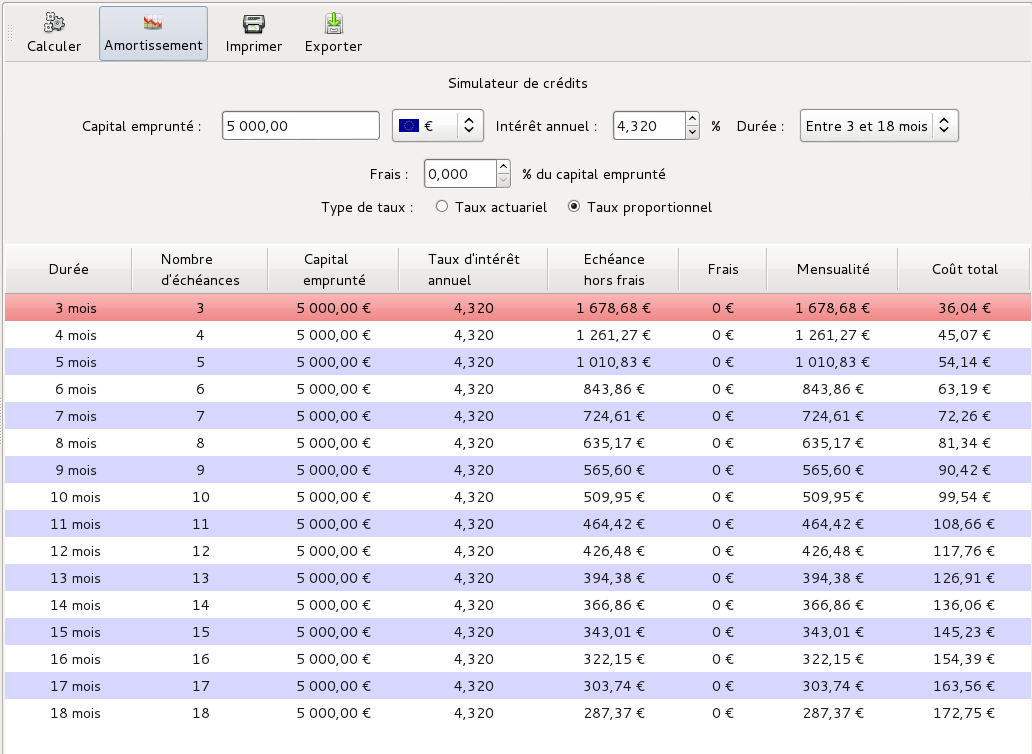
\includegraphics[scale=0.5]{image/screenshot/credit_simulation}
\end{center}
\caption{Simulateur de crédits}
\label{credit-simulation-img}
\end{figure}
% image centrée
\fi
 
Le simulateur de crédits se compose de deux éléments :
\begin{itemize}
	 \item la définition du crédit ; 
	 \item la liste des crédits simulés.
\end{itemize}


\subsection{Définition du crédit\label{credit-simulation-definition}}

La \menu{Définition du crédit} s'affiche en haut du panneau des détails, sous la barre d'outils. Elle affiche et permet de définir les caractéristiques principales du crédit suivantes :

\begin{itemize}
	 \item le capital emprunté ; 
	 \item la devise du crédit ;
	 \item le taux d'intérêt annuel ;
	 \item la plage de durée du crédit ;
	 \item les frais, en pourcentage du capital emprunté ;
	 \item le type du taux appliqué.
\end{itemize}


\subsection{Liste des crédits simulés\label{credit-simulation-list}}

La liste des crédits simulés s'affiche en bas du panneau des détails, sous la  \menu{Définition du crédit}. Elle affiche les caractéristiques détaillées de tous les crédits dont la durée fait partie de la plage de durées choisie dans la définition du crédit. 

La liste affiche en haut la barre de libellés des colonnes. Vous pouvez \indexword{élargir ou rétrécir une colonne}\index{colonne !largeur} en cliquant sur le séparateur entre deux colonnes et en le déplaçant. 

%XXXXXX Ne fonctionne pas  : XXXXXX Pour rétablir la largeur des colonnes à leur valeur par défaut, sélectionnez le menu \menu{Affichage - Réinitialiser la largeur des colonnes}.
%XXXXXX Ne fonctionne pas  : XXXXXX

%espace pour changement de thème
\vspacepdf{5mm}
La liste des crédits simulés affiche autant de lignes qu'il y a de durées de crédits possibles dans la plage de durées choisie dans la définition du crédit. Ses champs d'affichage sont les suivants :

\begin{itemize}
	 \item \menu{Durée} ;
	 \item \menu{Nombre d'échéances} ;
	 \item \menu{Capital emprunté} ;
	 \item \menu{Taux d'intérêt annuel} ;
	 \item \menu{Montant de l'échéance hors frais} ;
	 \item \menu{Montant des frais} ;
	 \item \menu{Mensualité} ;
	 \item \menu{Coût total du crédit}.
\end{itemize}

% espace pour changement de thème
\vspacepdf{5mm}
Vous pouvez déplacer la liste des crédits vers le haut ou vers le bas avec la molette de la souris, ou bien avec la souris et l'ascenseur vertical. 

%XXXXXX Ne fonctionne pas  : XXXXXXLe déplacement éventuel vers la gauche ou la droite se fait avec la souris et l'ascenseur horizontal.XXXXXX Ne fonctionne pas  : XXXXXX

Chaque crédit est affiché sur une ligne. Pour une bonne lisibilité de l'affichage, Grisbi présente une alternance de couleurs de fond violet et blanc{\couleurs} à chaque ligne.

%espace pour changement de thème
\vspacepdf{5mm}
Pour sélectionner un crédit, vous avez deux moyens :
\begin{itemize}
	 \item cliquez sur une de ses lignes ;
	 \item déplacez la sélection avec les touches du clavier \key{Flèche Haut}, \key{Flèche Bas}.
\end{itemize}
La ligne apparaît alors sur fond rouge{\couleur}.

%espace pour changement de thème
\vspacepdf{5mm}
Un menu contextuel est disponible par un clic-droit sur une ligne, et propose les actions suivantes :
\begin{itemize}
	 \item \menu{Afficher le tableau d'amortissement} ;
	 \item \menu{Imprimer le tableau} ;
	 \item \menu{Exporter le tableau}.
\end{itemize}


\section{Tableau d'amortissement\label{credit-amortization}}


Pour afficher les détails des amortissements, sélectionnez \menu{Amortissement} dans la barre 
\ifIllustration d'outil\refimage{credit-amortization-img}.
\else d'outils.
\fi

\ifIllustration
% image centrée 
\begin{figure}[tbp]
\begin{center}
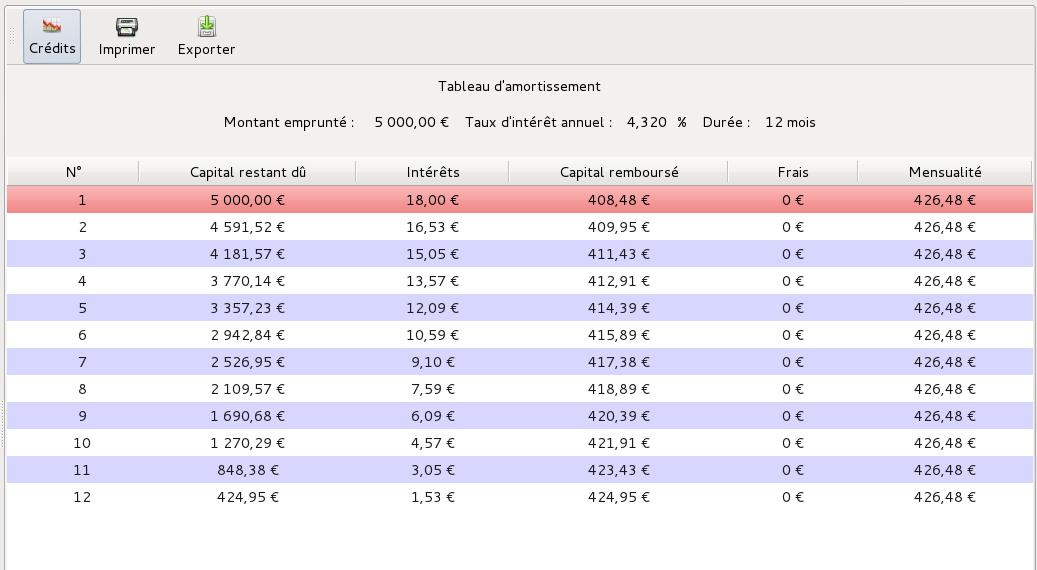
\includegraphics[scale=0.5]{image/screenshot/credit_amortization}
\end{center}
\caption{Tableau d'amortissement}
\label{credit-amortization-img}
\end{figure}
% image centrée
\fi

Le tableau d'amortissement se compose de deux éléments :
\begin{itemize}
	 \item la définition du crédit ; 
	 \item le tableau d'amortissement détaillé.
\end{itemize}


\subsection{Définition du crédit\label{credit-amortization-definition}}

La définition du crédit s'affiche en haut du panneau des détails, sous la barre d'outils. Elle affiche, \emph{mais ne permet pas de définir}, les caractéristiques principales du crédit suivantes :

\begin{itemize}
	 \item le montant emprunté ; 
	 \item le taux d'intérêt annuel ;
	 \item la durée du crédit.
\end{itemize}


\subsection{Tableau d'amortissement détaillé\label{credit-amortization-details}}

Le tableau d'amortissement détaillé s'affiche en bas du panneau des détails, sous la \menu{Définition du crédit}. Il affiche les caractéristiques détaillées de chaque échéance d'un crédit dont les caractéristiques principales sont affichées dans la définition du crédit juste au-dessus, et qui a été sélectionné dans la liste des crédits. 

Il affiche en haut la barre de libellés des colonnes. Vous pouvez \indexword{élargir ou rétrécir une colonne}\index{colonne !largeur} en cliquant sur le séparateur entre deux colonnes et en le déplaçant. 

%XXXXXX Ne fonctionne pas  : XXXXXX Pour rétablir la largeur des colonnes à leur valeur par défaut, sélectionnez le menu \menu{Affichage - Réinitialiser la largeur des colonnes}.
%XXXXXX Ne fonctionne pas  : XXXXXX

%espace pour changement de thème
\vspacepdf{5mm}
Le tableau d'amortissement affiche autant de lignes qu'il y a d'échéances dans le crédit choisi. Ses champs d'affichage sont les suivants :

\begin{itemize}
	 \item \menu{Numéro de l'échéance} ;
	 \item \menu{Capital restant dû} ;
	 \item \menu{Montant des intérêts} ;
	 \item \menu{Capital remboursé} ;
	 \item \menu{Montant des frais} ;
	 \item \menu{Mensualité}.
\end{itemize}

% espace pour changement de thème
\vspacepdf{5mm}
Vous pouvez déplacer la liste des échéances vers le haut ou vers le bas avec la molette de la souris, ou bien avec la souris et l'ascenseur vertical. 

%XXXXXX Ne fonctionne pas  : XXXXXX
%Le déplacement vers la gauche ou la droite se fait avec la souris et l'ascenseur horizontal.
%XXXXXX Ne fonctionne pas  : XXXXXX

Chaque échéance est affichée sur une ligne. Pour une bonne lisibilité de l'affichage, Grisbi présente une alternance de couleurs de fond violet et blanc{\couleurs} à chaque ligne.

%espace pour changement de thème
\vspacepdf{5mm}
Pour sélectionner une échéance, vous avez deux moyens :
\begin{itemize}
	 \item cliquez sur une de ses lignes ;
	 \item déplacez la sélection avec les touches du clavier \key{Flèche Haut}, \key{Flèche Bas}, \key{Page Haut}et \key{Page Bas}.
\end{itemize}
La ligne apparaît alors sur fond rouge{\couleur}.

%espace pour changement de thème
\vspacepdf{5mm}
Un menu contextuel est disponible par un clic-droit sur une ligne, et propose les actions suivantes :

\begin{itemize}
	 \item \menu{Afficher le simulateur de crédits} : affiche la zone de définition du crédit et la liste des crédits possibles ;
	 \item \menu{Imprimer le tableau} ;
	 \item \menu{Exporter le tableau}.
\end{itemize}


\section{Simulation d'un nouveau crédit\label{credit-new}}


Pour avoir accès à la simulation d'un nouveau crédit, cliquez sur \menu{Crédits} dans la barre d'outils (si cette fonction n'apparaît pas, c'est que le simulateur de crédits est déjà affiché).

% espace avant Attention ou Note  : 5 mm
\vspacepdf{5mm}
\textbf{Note} : À l'ouverture du simulateur de crédits, Grisbi affiche dans le pavé des détails les paramètres de définition du crédit et la liste des crédits générés lors d'une simulation précédente.
% espace après Attention ou Note  : 5 mm
\vspacepdf{5mm}

Pour simuler un nouveau crédit, entrez ses paramètres dans la définition du crédit :
\begin{itemize}
	 \item \menu{Capital emprunté} : le montant emprunté dans le champ de saisie, et sa devise dans la liste déroulante  ; 
	 \item \menu{Intérêt annuel} : le taux d'intérêt annuel dans le champ de saisie ou à l'aide de l'incrémenteur ;
	 \item \menu{Plage de durée} : la plage de durée du crédit dans la liste déroulante, ce qui va vous permettre de comparer les crédits ;
	 \item \menu{Frais} : les frais, en pourcentage du capital emprunté, dans le champ de saisie ou à l'aide de l'incrémenteur ; pour plus de précision de calcul, vous pouvez saisir jusqu'à trois décimales ;
	 \item \menu{Type du taux} : le type du taux appliqué, avec les boutons \menu{Taux actuariel} ou  \menu{Taux proportionnel} ; pour plus de précision de calcul, vous pouvez saisir jusqu'à trois décimales.
\end{itemize}

% espace avant Attention ou Note  : 5 mm
\vspacepdf{5mm}
\textbf{Note} : le taux d'intérêt est dit \indexword{taux actuariel}\index{taux !actuariel} lorsque les intérêts sont versés à la fin de la période annuelle ; le \indexword{taux proportionnel}\index{taux !proportionnel} est le taux nominal divisé par une unité de temps ; par exemple, le taux proportionnel mensuel est égal au taux nominal annuel divisé par 12.
% espace après Attention ou Note  : 5 mm
\vspacepdf{5mm}

La liste des crédits se met à jour automatiquement et affiche tous les crédits possibles en fonction de leur durée. 

Pour afficher le tableau d'amortissement de l'un des crédits, vous avez  deux moyens :

\begin{itemize}
	 \item sélectionnez-le, puis sélectionnez \menu{Amortissement} dans la barre d'outils ; 
	 \item cliquez-droit sur sa ligne, puis sélectionnez \menu{Afficher le tableau d'amortissement} dans le menu contextuel.
\end{itemize}

% espace avant Attention ou Note  : 5 mm
\vspacepdf{5mm}
\textbf{Note} : Grisbi n'enregistre pas le résultat des différentes simulations de crédit que vous avez faites : il enregistre uniquement dans le fichier de comptes les paramètres de définition du crédit saisis pour la dernière simulation ; il peut alors la rejouer ultérieurement ; pour conserver indéfiniment ces paramètres, utilisez les fonctions \menu{Imprimer} et \menu{Exporter}, explicitées ci-dessous.


\section{Export d'une simulation de crédits ou d'un tableau d'amortissement\label{credit-export}}


Grisbi vous permet d'exporter ces données, soit pour les enregistrer, soit pour les importer dans une autre application, par exemple un tableur pour y faire des calculs spécifiques.

Pour exporter une simulation de crédits ou un tableau d'amortissement, procédez comme suit :

\begin{enumerate}
	 \item dans la page \menu{Simulateur de Crédit} ou \menu{Tableau d'amortissement}, cliquez sur l'outil \menu{Exporter} dans la barre d'outils ; ou bien cliquez-droit sur une des lignes du tableau, puis sélectionnez \menu{Exporter le tableau} dans le menu contextuel ; une fenêtre de gestionnaire de fichiers s'affiche ;
	 \item saisissez le nom du fichier à exporter, dont l'extension sera \file{.csv} ;
	 \item choisissez son répertoire de destination ;
	 \item cliquez sur le bouton \menu{Enregistrer}.
\end{enumerate}

% espace avant Attention ou Note  : 5 mm
\vspacepdf{5mm}
\strong{Attention} : d'une manière générale, il est déconseillé d'avoir des accents ou des espaces dans les noms des répertoires et fichiers utilisés par Grisbi. Si c'est le cas, renommez-les maintenant. Par exemple, les espaces peuvent être remplacées par des tirets bas (\_).


\section{Impression d'une simulation de crédits ou d'un tableau d'amortissement\label{credit-print}}


Pour imprimer une simulation de crédits ou un tableau d'amortissement, procédez comme suit :

\begin{enumerate}
	 \item dans la page \menu{Simulateur de Crédit} ou \menu{Tableau d'amortissement}, cliquez sur le bouton \menu{Imprimer} de la barre d'outils, ou bien cliquez-droit sur une des lignes du tableau, puis sélectionnez \menu{Imprimer le tableau} dans le menu contextuel ;
	 \item  une fenêtre d'impression s'ouvre, dont l'aspect et les fonctions dépendent de votre gestionnaire d'impression ; vous aurez le plus souvent les choix suivants :
		  \begin{itemize}
			  \item imprimer dans un fichier (en format \indexword{\gls{PostScript}}\index{postscript}, \indexword{\gls{PDF}}\index{pdf} ou \indexword{\gls{SVG}}\index{svg}) ; 
			  \item imprimer avec votre imprimante.
		  \end{itemize}
\end{enumerate}

% espace pour changement de thème
\vspacepdf{5mm}
En fonction de votre gestionnaire d'impression, vous pourrez disposer de réglages divers tels que la taille et l'orientation de la feuille, la résolution, la police d'impression et sa taille, etc.
